\section{$\Delta$QSD implementation}
    In this section we provide the mathematical foundations of $\Delta$QSD as they are implemented in the oscilloscope.
    \subsection{Histogram representation of $\Delta$Q}
    We approximate the probability distribution of $\Delta$Q via histograms.
   \subsubsection{PDF}
   We partition the values into $N$ bins of equal width, Given $\lbrack x_i, x_{i+1} \rbrack$ the interval of a bin $i$, where $x_i = i\Delta t$, and $\hat{p}(x_i)$ the value of the PDF at bin $i$, for $n$ bins:
        \begin{equation}
            \begin{cases}
                \hat{p}(i) = \dfrac{s_i}{n}, \text{if } i \le n \\
                \hat{p}(i) = 0, \text{if } i > n \\
            \end{cases}
            \label{eq:pdf}
        \end{equation}
    Where $s_i$ the number of successful outcome instances whose elapsed time is contained in the bin $i$, $n$ the total number of instances. \cite{stat}

    \subsubsection{CDF}
        The value $x_i = \hat{f}(i)$ of the CDF at bin $i$ with $n$ bins can be calculated as:
        \begin{equation}
            \begin{cases}
                \hat{f}(i) = \sum_{j=1}^{i} \hat{p}(j), & \text{if } i \le n \\  
                \hat{f}(i) = \hat{f}(n), & \text{if } i > n 
            \end{cases}
            \label{eq:cdf}
        \end{equation}
 
    \begin{figure}[H]
            \begin{center}
                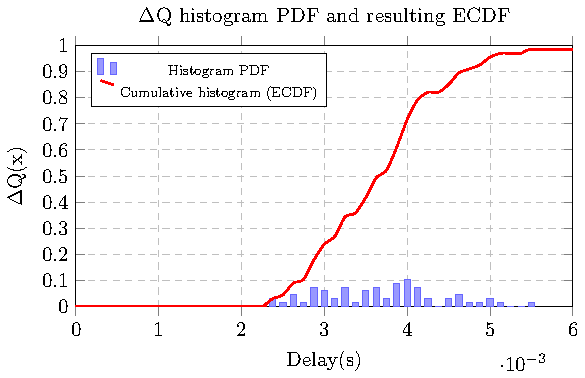
\includegraphics[scale=1]{tikz/pdf_dq.pdf} 
            \end{center}
            \caption{Blue bins: PDF of a sample $\Delta$Q. Red: Resulting CDF of $\Delta$Q PDF, the CDF is what is displayed on the dashboard.}
        \end{figure}

    \subsection{dMax}
        We introduced $dMax$ in the previous chapters (\cref{eq:dMaxU}), we provide here the full equation that allows $dMax$ to be calculated:
        \begin{equation}
            \begin{split}
                \Delta t &= \Delta t_{base} \cdot 2^n \\ 
                dMax &= \Delta t_{base} \cdot 2^n \cdot N  
            \end{split}
            \label{eq:dMaxU}
        \end{equation}
        Where:
        \begin{itemize}
            \item $\Delta t_{base}$ represents the base width of a bin, equal to 1ms.
            \item $n$ the exponent that is set by the user in the dashboard. It is limited to [-10, 10].
            \item $N$ the number of bins, it is limited to [1, 1000].
        \end{itemize}
            We chose 1 ms in combination with $2^n$ as it allows us to go from very fine bin widths ($\approx$ 1 $\mu$s) to large bin widths ($\approx$ 1 s), thanks to the [-10, 10] bounds. Moreover, scaling by a power of 2 allows all the probe's $\Delta$Qs to have a common factor to perform operations on them after rebinning (\cref{eq:rebin}).

   \subsection{Rebinning}
            Rebinning refers to the aggregation of multiple bins of a bin width $i$ to another bin width $j$ \cite{rebin}. 
            Previous operations between $\Delta$Qs must be done on $\Delta$Qs that have the same bin width. This is why it is fundamental that all probes have a common $\Delta t_{base}$ and why we have a $2^n$ factor to calculate the total bin width.

            Given two $\Delta$Qs $\Delta$Q$_i$, $\Delta$Q$_j$, the common bin width $\Delta t_{ij}$ is:
            \begin{center}
                $\Delta t_{ij}$ = max \{$\Delta t_i, \Delta t_j \}$
            \end{center}
            The PDF of the rebinned $\Delta$Q at bin $b$, from the original PDF of $n$ bins, where $\Delta t_i > \Delta t_j$ and k = $\frac{\Delta t_i}{\Delta t_j}$:
            \begin{equation}
                p'_b = \sum_{n=b \cdot k}^{b+ 1 \cdot k - 1} p_n, \quad b=0,1,\dots \lceil \frac{N}{k} \rceil  
                \label{eq:rebin}
            \end{equation}
            We perform rebinning to a higher bin width for a simple reason. While this leads to loss of information for the $\Delta$Q with the lowest bin width, rebinning to a lower bin width would imply inventing new values for the $\Delta$Q with the highest bin width.
        \begin{figure}[H]
            \centering
            \begin{subfigure}{.5\textwidth}
                \centering
                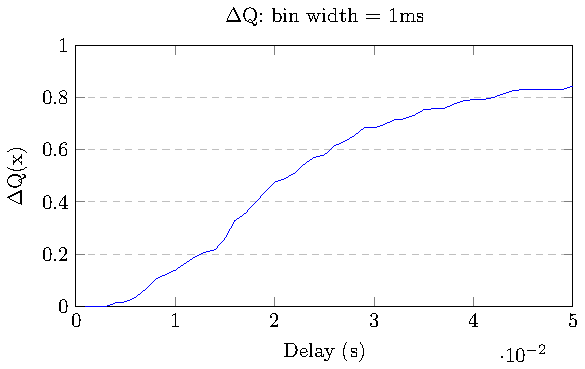
\includegraphics[width =0.98\textwidth]{tikz/cdf.pdf}
                \label{fig:nrb}
                \subcaption{Sample $\Delta$Q with 1ms bins}%
            \end{subfigure}%
            \begin{subfigure}{.5\textwidth}%
                \centering%
                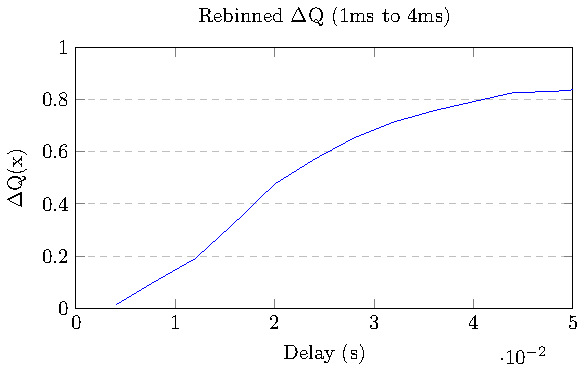
\includegraphics[width =0.98\textwidth]{tikz/rebinned_cdf.pdf}%
                \label{fig:sub2}%
                \subcaption{$\Delta$Q on the left after rebinning to 4ms bins}%
            \end{subfigure}%
            \label{fig:w1w2hb}%
            \end{figure}%

    \subsection{Convolution} \label{convol}
    We present the two solutions to perform convolution we explored during the implementation.  
        \subsubsection{Naïve convolution}
        Given two $\Delta$Q binned PDFs $f$ and $g$ with equal bin widths, the result of the convolution $f \circledast g$ is given by \cite{conv}: 
        \begin{equation}
            (f \circledast g)\lbrack n \rbrack = \sum_{m = 0}^{N} = f\lbrack m \rbrack g \lbrack n - m \rbrack  
            \label{eq:discconv}
        \end{equation}

        The naïve way of calculating convolution has a time complexity of $\mathcal{O}(N^2)$, this quickly becomes a problem as soon as the user wants to have a more fine-grained understanding of a component. The oscilloscope presented noticeable lag and frame skipping with high resolution. This is why we decided to explore Fast Fourier Transform convolution. 
 
    \subsubsection{Fast Fourier Transform Convolution}
        FFTW (Fastest Fourier Transform in the West) is a C subroutine library \cite{fftw3} for computing the discrete Fourier Transform in one or more dimensions, of arbitrary input size, and of both real and complex data. We use FFTW in our program to compute the convolution of $\Delta$Qs. We adapt our script from an already existing one found on GitHub. \cite{fft}
    
    Whilst the previous algorithm is far too slow to handle a high number of bins, convolution leveraging Fast Fourier Transform (FFT) allows us to reduce the amount of calculations to $\mathcal{O}(N \text{log} N)$. This is why the naïve convolution algorithm is not used. We will analyse the time gains in Chapter 7.
    
    FFT and naïve convolution produce the same results in our program, barring $\varepsilon$ differences (around $10^{-18}$) in bins whose result should be 0. This is most likely due to rounding error.
    
    FFTs algorithms are plenty, the choice of the one to use is left up to the subroutine via the parameter \texttt{FFTW\_ESTIMATE}. \cite{fft-h}
    
    The explanation of the algorithm is beyond the scope of this master thesis, we refer the reader to the following book as a reference. \cite{fft-book}

    \subsection{Arithmetical operations}
        The FTF, ATF and PC operators on $\Delta$Qs use a simple set of arithmetical operations to calculate a $\Delta$Q.   
    The time complexity of FTF, ATF and PC is trivially $\mathcal{O}(N)$ where N is the number of bins.
 
    \paragraph{Scaling (multiplication)} A $\Delta$Q can be scaled w.r.t. a constant $0 \le j \le 1$. It is equal to binwise multiplication on CDF bins. It is used for the probabilistic choice operator.
    \begin{equation}
        \hat{f_r}(i) = \hat{f}(i) \cdot j
        \label{eq:mul_ecdf}
    \end{equation}

    \paragraph{Operations between $\Delta$Qs} 
        Addition, subtraction and multiplication can be done between two $\Delta$Q of equal bin width (but not forcibly of equal length) by calculating the operation between the two CDFs of the $\Delta$Qs:
        \begin{equation}
            \Delta \text{Q}_{AB}(i) = \hat{f_A}(i) [\cdot, +, -] \hat{f_B}(i)
            \label{eq:op_dq}
        \end{equation}
    They are used for all operators.

    \subsection{Confidence bounds}
        Here is how we calculate the mean and lower/upper confidence for the $\Delta$Qs CDF at bin $i \quad \forall i < N$. \cite{stat}

        For $x_{ij}$, the value of an CDF $j$ at bin $i$, the mean of $n$ CDFs for the bin $i$ in a polling window is:
            \begin{equation}
                \mu_i = \dfrac{1}{n} \sum_{j=1}^{n} x_{ij}
                \label{eq:mean_ecdf}
            \end{equation}
        Its variance:
            \begin{equation}
                \sigma^2_i = \dfrac{1}{n} \sum_{j=1}^{n} x^2_{ij} - \mu^2_i
                \label{eq:var_ecdf}
            \end{equation}
        The lower confidence bound $CI_{i, l}$ and upper confidence bound $CI_{i, u}$ for a bin $i$ can be calculated as:
        \begin{equation}
                CI_{i, l} = \mu_i - \dfrac{\sigma_i}{\sqrt{n}} \ \text{,} \ CI_{i, u} = \mu_i + \dfrac{\sigma_i}{\sqrt{n}}
            \label{eq:ci_i}
        \end{equation}
        The confidence bounds for the cdf are the lower and confidence bounds for every bin $i$.

     
